\chapter{Dasar Teori}
\label{chap:Dasar Teori}

\section{jsoup}
\label{sec:jsoup}

\textit{Web scraping}\cite{Vargiu:2013} adalah teknik mendapatkan informasi dari sebuah situs web secara otomatis. Dalam Java, \textit{web scraping} dapat diimplementasikan menggunakan \textit{library} jsoup\cite{jsoup}. API yang disediakan oleh jsoup dapat digunakan untuk mengekstrak dan memanipulasi data HTML. 

Subbab-subbab berikut menjelaskan kelas-kelas dari jsoup yang terkait dengan pengerjaan skripsi ini.

\subsection{Jsoup}

Kelas ini merupakan inti untuk mengakses fungsi jsoup. Salah satu \textit{method} yang dimiliki kelas ini adalah sebagai berikut:
\begin{itemize}
	\item \textbf{public static Connection connect(String url)} \\
		Berfungsi untuk membuat koneksi baru dengan suatu situs web. \\
		\textbf{Parameter:}
		\begin{itemize}
			\item \textbf{url} URL situs web dengan protokol HTTP atau HTTPS.
		\end{itemize}
		\textbf{Kembalian:} koneksi dengan situs web.
\end{itemize}

\subsection{Connection}

Kelas ini merupakan interface yang menyediakan pengambilan data dari situs web. Beberapa \textit{method} yang dimiliki kelas ini adalah sebagai berikut:

\begin{itemize}
	\item \textbf{Connection cookies(Map<String,String> cookies)} \\
		Berfungsi untuk menambahkan \textit{cookie}. \\
		\textbf{Parameter:}
		\begin{itemize}
			\item \textbf{cookies} \textit{map} dari \textit{cookie}.
		\end{itemize}
		\textbf{Kembalian:} koneksi dengan situs web.
		
		\item \textbf{Connection data(String key, String value)} \\
		Berfungsi untuk menambahkan parameter data. \\
		\textbf{Parameter:}
		\begin{itemize}
			\item \textbf{key} kunci data.
			\item \textbf{value} nilai data.
		\end{itemize}
		\textbf{Kembalian:} koneksi dengan situs web.
		
		\item \textbf{Connection method(Connection.Method method)} \\
		Berfungsi untuk mengatur metode pengiriman. \\
		\textbf{Parameter:}
		\begin{itemize}
			\item \textbf{method} metode pengiriman HTTP \textit{request}.
		\end{itemize}
		\textbf{Kembalian:} koneksi dengan situs web.
		
		\item \textbf{Connection timeout(int millis)} \\
		Berfungsi untuk mengatur batas waktu \textit{request}. Batas waktu nol akan dianggap sebagai batas waktu yang tak terhingga. \\
		\textbf{Parameter:}
		\begin{itemize}
			\item \textbf{millis} banyaknya milisekon sebelum batas waktu.
		\end{itemize}
		\textbf{Kembalian:} koneksi dengan situs web.
		
		\item \textbf{Connection validateTLSCertificates(boolean value)} \\
		Berfungsi untuk mengatur pemeriksaan sertifikat TLS untuk HTTPS \textit{request}. Nilai "`true"' untuk memeriksa dan nilai "`false"' untuk tidak memeriksa.\\
		\textbf{Parameter:}
		\begin{itemize}
			\item \textbf{value} status pemeriksaan sertifikat TLS.
		\end{itemize}
		\textbf{Kembalian:} koneksi dengan situs web.
		
		\item \textbf{Connection.Response execute()} \\
		Berfungsi untuk mengirim \textit{request}.\\
		\textbf{Kembalian:} objek Response.	
\end{itemize}

\subsection{Response}

Kelas ini merepresentasikan HTTP \textit{response}. Response merupakan turunan dari kelas Base yang menangani response dan \textit{request}. Beberapa \textit{method} yang dimiliki kelas ini adalah sebagai berikut:
\begin{itemize}
	\item \textbf{Map<String,String> cookies()} \\
		\textit{Method} ini diturunkan dari kelas Base, berfungsi untuk mendapatkan seluruh \textit{cookies}. \\
		\textbf{Kembalian:} seluruh \textit{cookies}.	
		
		\item \textbf{Document parse()} \\
		Berfungsi untuk \textit{parsing} \textit{response body} menjadi dokumen. \\
		\textbf{Kembalian:} koneksi dengan situs web.
		
		\item \textbf{String body()} \\
		Berfungsi untuk mendapatkan \textit{response body} berupa \textit{string}. \\
		\textbf{Kembalian:} \textit{response body} dalam bentuk \textit{string}.
\end{itemize}

\subsection{Document}

Kelas ini merepresentasikan dokumen HTML. Salah satu \textit{method} yang dimiliki kelas ini adalah sebagai berikut:
\begin{itemize}
	\item \textbf{public Elements select(String cssQuery)} \\
		\textit{Method} ini diturunkan dari kelas Element, berfungsi untuk menemukan elemen HTML yang sesuai dengan kueri CSS. \\
		\textbf{Parameter:} 
		\begin{itemize}
			\item \textbf{cssQuery} kueri CSS.
		\end{itemize}
		\textbf{Kembalian:} elemen-elemen HTML yang sesuai dengan kueri CSS.	
\end{itemize}

\subsection{Elements}

Kelas ini merepresentasikan kumpulan elemen HTML. Beberapa \textit{method} yang dimiliki kelas ini adalah sebagai berikut:
\begin{itemize}
	\item \textbf{public Elements select(String query)} \\
		\textit{Method} Berfungsi untuk menemukan elemen-elemen yang sesuai dalam \textit{list} elemen. \\
		\textbf{Parameter:} 
		\begin{itemize}
			\item \textbf{query} kueri \textit{Selector}.
		\end{itemize}
		\textbf{Kembalian:} elemen-elemen yang sudah diseleksi sesuai kueri.	
		
		\item \textbf{public String val()} \\
		\textit{Method} Berfungsi untuk mendapatkan nilai dari elemen pertama. \\
		\textbf{Kembalian:} nilai elemen.	
		
		\item \textbf{public String text()} \\
		\textit{Method} Berfungsi untuk mendapatkan kombinasi teks dari seluruh elemen yang sesuai. \\
		\textbf{Kembalian:} seluruh teks dalam \textit{string}.	
\end{itemize}

\subsection{Element}

Kelas ini merepresentasikan sebuah elemen HTML yang berisikan \textit{tag}, atribut, dan \textit{child}. Beberapa \textit{method} yang dimiliki kelas ini adalah sebagai berikut:
\begin{itemize}
	\item \textbf{public Element child(int index)} \\
		\textit{Method} Berfungsi untuk mendapatkan \textit{child element} berdasarkan nomor indeks. \\
		\textbf{Parameter:} 
		\begin{itemize}
			\item \textbf{index} nomor index.
		\end{itemize}
		\textbf{Kembalian:} \textit{child element}.	
		
		\item \textbf{public Element child()} \\
		\textit{Method} Berfungsi untuk mendapatkan seluruh \textit{child element}. \\
		\textbf{Kembalian:} seluruh \textit{child element}.	
		
		\item \textbf{public String className()} \\
		\textit{Method} Berfungsi untuk mendapatkan nama kelas elemen. \\
		\textbf{Kembalian:} nama kelas elemen.	
		
		\item \textbf{public String text()} \\
		\textit{Method} Berfungsi untuk mendapatkan teks dari elemen. \\
		\textbf{Kembalian:} teks dalam \textit{string}.	
\end{itemize}



\section{Chrome DevTools}
\label{sec:devtools}

Chrome Developer Tools (DevTools)\cite{devtools} adalah perangkat \textit{debugging} yang dimiliki Google Chrome. Saat menunjungi suatu halaman web, pengguna DevTools dapat melakukan \textit{debugging} pada halaman tersebut. DevTools dapat diakses dengan menekan "`Ctrl+Shift+I"' saat sedang membuka suatu halaman web.  

Panel-panel yang dimiliki DevTools (Gambar \ref{fig:2_chrome_devtools}) antara lain:
\begin{enumerate}
	\item \textbf{Elements}, memeriksa dan mengubah elemen HTML dan \textit{style} dari suatu situs web.
	\item \textbf{Console}, mendapatkan informasi pengembangan dan berinteraksi dengan dokumen.
	\item \textbf{Sources}, melakukan \textit{debugging} pada JavaScript dengan menentukan \textit{breakpoint}.
	\item \textbf{Network}, memantau kinerja jaringan pada \textit{website} secara \textit{real-time}.
	\item \textbf{Audits}, menganalisa halaman yang dimuat.
	\item \textbf{Timeline}, menampilkan alur waktu saat memuat halaman.
	\item \textbf{Profiles}, menggambarkan waktu eksekusi dan penggunaan memori saat memuat halaman.
	\item \textbf{Resources}, memeriksa sumber daya halaman yang dapat berupa basis data, \textit{cookies}, dan \textit{cache}.
\end{enumerate}

\begin{figure}[H]
	\centering
	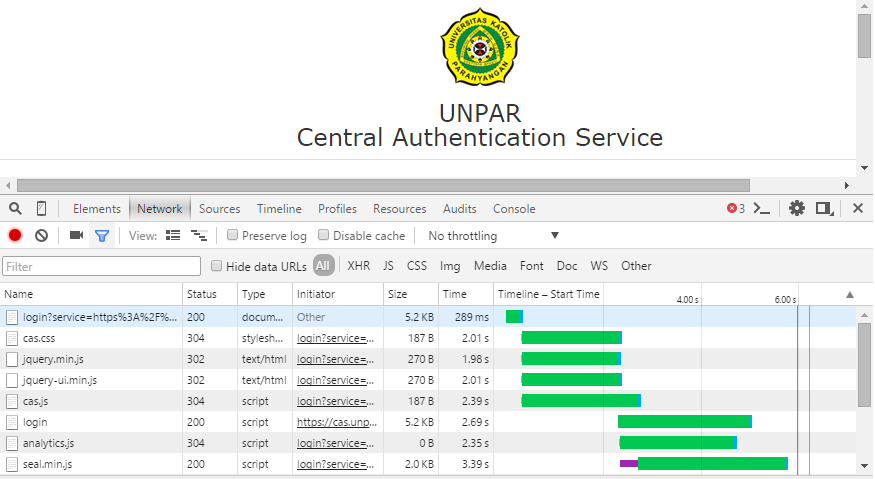
\includegraphics[scale=0.5]{Gambar/chrome-devtools}
	\caption{Chrome DevTools} 
	\label{fig:2_chrome_devtools}
\end{figure}

Pada subbab-subbab berikut akan dijelaskan mengenai dua panel dari DevTools.

\subsection{Elements}
Panel Elements memungkinkan untuk memperlihatkan informasi yang terstruktur tentang halaman yang sedang dibuka. HTML akan ditampilkan dalam bentuk pohon \textit{Document Object Model} (DOM). Tampilan pohon DOM memperlihatkan struktur DOM dari halaman yang sedang dibuka. Pohon DOM adalah pohon dari node-node yang mewakili setiap elemen HTML seperti \texttt{<body>} dan \texttt{<p>}. Tampilan struktur pohon DOM menampilkan tag elemen HTML bukan jenis node DOM. Misalnya, \texttt{<p>} bukan \texttt{HTMLParagraphElement}. 

Pemeriksaan elemen akan memperlihatkan node DOM dan CSS dari elemen yang dipilih pada \textit{browser}. Pemeriksaan elemen dapat dilakukan dengan cara klik kanan pada elemen yang ingin diperiksa kemudian pilih "`Inspect element"'. Dengan melakukan pemeriksaan elemen, jendela panel Elements akan muncul (Gambar \ref{fig:2_elements_panel}). 

\begin{figure}[H]
	\centering
	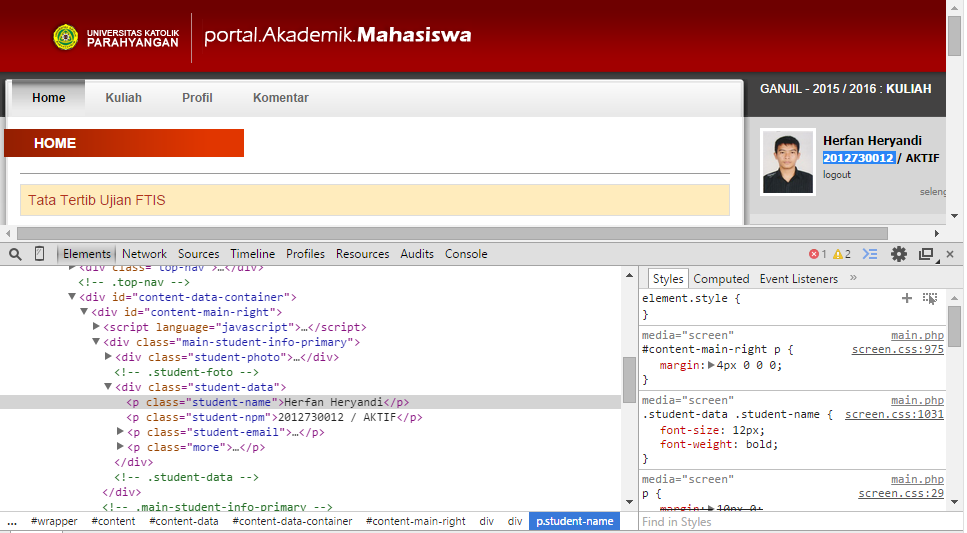
\includegraphics[scale=0.5]{Gambar/elements-panel}
	\caption{Panel Elements} 
	\label{fig:2_elements_panel}
\end{figure}

\subsection{Network}
Panel Network secara otomatis mencatat semua aktivitas jaringan saat DevTools terbuka. Pertama kali dibuka, panel Network masih kosong. Halaman web harus dimuat ulang untuk mulai mencatat aktivitas jaringan atau menunggu adanya aktivitas jaringan pada halaman web. Setiap \textit{resource} yang dicatat akan ditambahkan ke dalam sebuah baris dalam tabel Network. Sedangkan kolom dari tabel Network berisi:
\begin{itemize}
	\item \textbf{Name dan Path}, nama dan URL dari \textit{resource}.
	\item \textbf{Method}, HTTP \textit{request method}.
	\item \textbf{Status dan Text}, kode status HTTP dan pesan.
	\item \textbf{Domain}, domain dari \textit{resource}.
\end{itemize}

%skip%

Ketika nama \textit{resource} dalam tabel Network diklik, maka akan muncul tab baru. Beberapa detail dari tab baru tersebut adalah sebagai berikut:
\begin{itemize}
	\item \textbf{Header}\\
	\item \textbf{Preview}\\
	\item \textbf{Response}\\
	\item \textbf{Cookies}\\
\end{itemize}

\section{Play Framework}
\label{sec:play}

Play Framework \cite{Leroux:2014} merupakan sebuah web framework berbasis Java dan Scala. Play juga menggunakan \textit{design pattern} Model-View-Controller (MVC) di mana \textit{model} dan \textit{controller} menggunakan Java sedangkan \textit{view} menggunakan Scala dan HTML. 
